% This is LLNCS.DEM the demonstration file of
% the LaTeX macro package from Springer-Verlag
% for Lecture Notes in Computer Science,
% version 2.4 for LaTeX2e as of 16. April 2010
%
\documentclass{iacrtrans}
\usepackage{epstopdf}
\usepackage[T1]{fontenc}
\usepackage{lmodern}
\usepackage{relsize}
\usepackage[utf8]{inputenc}
\usepackage[compatibility=false]{caption}
\usepackage{subcaption}
\usepackage{pgf}
\usepackage{tikz}
\usetikzlibrary{arrows,automata}
\usepackage{tikz-timing}
\usepackage{todonotes}
\usepackage{tabularx}
\usepackage{microtype}
\usepackage{booktabs}
\usepackage{amsmath}
\usepackage{amssymb}
\usepackage{authblk}
\usepackage[hyphens]{url}
\usepackage{hyperref}
\hypersetup{breaklinks=true}
\usepackage{algorithm}
%\usepackage{algorithmic}
\usepackage{algpseudocode}
\usepackage{cite}
\usepackage{units}
%\usepackage{algpseudocode}
%\usepackage{algorithm2e}
%\usepackage[]{algorithm2e}
\usepackage{algpseudocode}
\usepackage{bm}
\usepackage{mathtools}
\usepackage{theorem}
\usepackage{mathrsfs}
\usepackage{listings}
\usepackage{cleveref}
\usepackage{pifont}
%\usepackage{refcheck}
\algnewcommand{\AND}{\algorithmicand}
\newcommand{\cmark}{\ding{51}}
\newcommand{\xmark}{\ding{55}}
\newcommand\numberthis{\addtocounter{equation}{1}\tag{\theequation}}
\newcommand{\eqd}{\ensuremath{=_{\mathrm{\scriptscriptstyle def}}}}
\newcommand{\Z}{\ensuremath{\mathbb Z}}
\newcommand\myE[1]{\ensuremath\mathbb{E}\left\lbrack #1 \right\rbrack} % The expectation (or mean, or esperance)
\newcommand\myV[1]{\ensuremath\mathsf{Var}\left\lbrack #1 \right\rbrack} % The variance
\newcolumntype{P}[1]{>{\centering\arraybackslash}p{#1}}
\setcounter{secnumdepth}{3}


\newcommand{\stodo}[1]{\todo[inline,caption={}]{TODO: #1}}
\newcommand{\minus}{\scalebox{0.75}[1.0]{$-$}}


%\newtheorem{theorem}{Theorem}
%\newtheorem{corollary}[theorem]{Corollary}
%\newtheorem{definition}[theorem]{Definition}
%\newtheorem{property}[theorem]{Property}
%\newtheorem{lemma}[theorem]{Lemma}

%%%% Special environments
%\newenvironment{proof}{\noindent \textbf{Proof}}{\qed \vskip 1em}
%\newcommand{\qed}{\hfill \ensuremath{\Box}}

%
\begin{document}
%

\title{Standard Lattice-Based Key Encapsulation\\ on Embedded Devices}

\author{
James Howe\textsuperscript{1}, Tobias Oder\textsuperscript{2}, Markus Krausz\textsuperscript{2}, and Tim G\"uneysu\textsuperscript{2,3}
}

\institute{
\textsuperscript{1}Department of Computer Science, University of Bristol, UK \texttt{james.howe@bristol.ac.uk}\\
\textsuperscript{2}Horst G\"ortz Institute for IT Security, Ruhr-Universit\"at Bochum, Germany \texttt{\{tobias.oder,markus.krausz,tim.gueneysu\}@rub.de}\\
\textsuperscript{3}DFKI, Germany\\
}

\keywords{Post-quantum cryptography, standard lattices, Frodo, KEM, FPGA, microcontroller, embedded security, hardware security.}

\maketitle

\begin{abstract} \label{abtract}
Lattice-based cryptography is one of the most promising candidates being considered to replace current public-key systems in the era of quantum computing. In 2016, Bos et al. proposed the key exchange scheme \textsf{FrodoCCS}, that is also a submission to the NIST post-quantum standardization process, modified as a key encapsulation mechanism (\textsf{FrodoKEM}). The security of the scheme is based on standard lattices and the learning with errors problem. Due to the large parameters, standard lattice-based schemes have long been considered impractical on embedded devices. The \textsf{FrodoKEM} proposal actually comes with parameters that bring standard lattice-based cryptography within reach of being feasible on constrained devices. In this work, we take the final step of efficiently implementing the scheme on a low-cost FPGA and microcontroller devices and thus making conservative post-quantum cryptography practical on small devices. 
Our FPGA implementation of the decapsulation (the computationally most expensive operation) needs 7,220 look-up tables (LUTs), 3,549 flip-flops (FFs), a single DSP, and only 16 block RAM modules. The maximum clock frequency is 162 MHz and it takes 20.7 ms for the execution of the decapsulation. Our microcontroller implementation has a 66\% reduced peak stack usage in comparison to the reference implementation and needs 266 ms for key pair generation, 284 ms for encapsulation, and 286 ms for decapsulation. Our results contribute to the practical evaluation of a post-quantum standardization candidate.
\end{abstract}
\section{Introduction}

Secure communications channels have become essential for the transmission of
sensitive information over the Internet or between embedded devices, requiring
protocols such as public-key encryption and digital signatures. Furthermore, these
requirements for data security and privacy are becoming more important as the number of connected devices increases, due to the popularity of the Internet of Things.

So far, practitioners have relied on cryptography based on the hardness of the
factoring assumption (RSA) or the discrete logarithm problem (ECC).
However, should a quantum computer be realized, the hardness of these related
problems will be seriously weakened. This issue not only affects future communications
but also secure messages sent today, which could be intercepted and
stored, then decrypted by a device built a decade from now. Preparing for this is
therefore paramount, and hence quantum-safe alternatives are needed to provide
long-term security. The National Institute for Standards and Technology (NIST) has called for quantum-resistant cryptographic algorithms for new public-key cryptography standards, similar to previous AES and SHA-3 competitions \cite{chen2016report}.

Lattice-based cryptography is one of the most promising replacements for classical cryptography, accounting for more than 40\% of the submissions to the NIST post-quantum standardization effort. This is due to many reasons, one of which is that most of the computations required involves very simple and parallelizable operations like integer multiplication, addition, and modular reduction. Unlike RSA-based schemes, which involve very hard computations like modular exponentiation. Moreover, lattice-based cryptography benefits from the strong security notion of worst-case to average-case hardness, meaning average-case instances are at least as hard as worst-case instances of related (much smaller) lattice problems \cite{DBLP:conf/crypto/MicciancioP13}.

In recent years, there has been tremendous growth in lattice-based cryptography as a research field. As a result, concepts such as functional encryption \cite{DBLP:conf/tcc/BonehSW11}, identity-based encryption \cite{DBLP:conf/asiacrypt/DucasLP14}, attribute-based encryption \cite{DBLP:conf/tcc/Boyen13}, and fully homomorphic encryption \cite{gentry2009fully} are now available. On the practical front, some constructions of public-key encryption schemes and digital signature schemes based on lattice problems are now more practical than traditional schemes based on RSA \cite{DBLP:journals/tecs/HowePOOG15}. Lyubashevsky \cite{DBLP:conf/pkc/Lyubashevsky08,DBLP:conf/eurocrypt/LyubashevskyPR10} proposed a new class of lattices, \textit{ideal} lattices, that provide higher efficiency than standard lattices as schemes based upon ideal lattices require less memory and have a better performance than schemes based on standard lattices. Therefore the majority of research targeting practical evaluations of lattice-based cryptography have focused on ideal lattices \cite{DBLP:conf/ches/GottertFSBH12, DBLP:conf/pqcrypto/GuneysuOPS13, ducas2013lattice, DBLP:conf/ches/RoyVMCV14,DBLP:journals/iacr/0001SRGKV15, DBLP:conf/cans/LongaN16,rtesla}. This improvement in efficiency is possible due to an introduced structure in the underlying lattice in these constructions. While the main operation in standard lattices is matrix-vector (or matrix-matrix) multiplication, the complexity is reduced to polynomial multiplication in ideal lattice-based cryptography. However, to this day it is not clear whether a future (quantum) attack might be able to exploit this additional structure, introduced in ideal lattices, in order to break the cryptosystem. Standard lattices do not suffer from this potential weakness and can therefore be considered the more conservative choice, as recommended by Howe et al. \cite{DBLP:conf/dac/HoweMORGB16} and the EU Horizon 2020 project PQCRYPTO \cite{initial}. The EU Horizon 2020 project SAFEcrypto also investigate the use of (standard) lattice-based cryptography in hardware, specifically for conservative use cases such as satellite communications.

The \textsf{FrodoCCS} key exchange scheme by Bos et al. \cite{DBLP:conf/ccs/BosCDMNNRS16} is designed to offer exactly this -- trading some efficiency for high security trust in the post-quantum era. Another design rationale for \textsf{FrodoCCS} is for simplicity, and this is seen in its use of basic operations like addition and multiplication. The parameter sets are much more flexible and easier to scale in comparison to \textsf{NewHope} variants \cite{DBLP:conf/uss/AlkimDPS16,NISTPQC-R1:NewHope17}, which have a number of restrictions in order to use NTT polynomial multiplication, and can target more security levels which essentially scale linearly.

A modified version of \textsf{FrodoCCS} \cite{DBLP:conf/ccs/BosCDMNNRS16} has been submitted to the NIST standardization process \cite{frodo-nist}, proposed as a key encapsulation mechanism (KEM), named \textsf{FrodoKEM}. The submission comes with a reference implementation and a vectorized implementation for high-end Intel CPUs. However, to date there has been no research into the feasibility of \textsf{Frodo} variants on embedded devices. In this paper, we want to bridge the gap between the lack of practical evaluations of standard lattice-based cryptography and the need for long-term security solutions for the Internet of Things. This task is especially challenging considering the conservative parameters that were a design rationale of \textsf{Frodo} variants. As embedded devices, like FPGAs and microcontrollers, usually have very limited memory, we have to pay special attention to minimize the memory consumption of our implementations while not deteriorating the performance too much to not overexert the limited computing capabilities of these platforms.

%This presentation focuses on \emph{practical} lattice-based cryptography, with an inclination towards hardware architectures and optimisations. The talk will survey the trends of past implementations of lattice-based designs, discuss the current state-of-the-art, and propose future research avenues that need to be addressed if lattice-based cryptography is to be integrated in real-world systems.

%Previous designs have mainly focused on highly optimised encryption and digital signatures schemes, as well as the modules used ubiquitously within the area such as number theoretic transform (NTT) multipliers and discrete Gaussian samplers. We will go in depth regarding the differences between these implementations and discuss the importance of each module with respect to the overall performance.

%With the NIST post-quantum standardisation project in its first stage, the main focus of cryptographers today is to evaluate the competing schemes with respect to cryptanalysis. Moreover, these schemes have (and will) come under scrutiny with respect to side-channel analysis (SCA). These current trends will also be discussed in the talk, outlining the potential weaknesses in lattice-based cryptosystems and the fixes proposed for them.

%This presentation will also touch on the importance of hardware designs, in particular on field-programmable gate arrays (FPGAs), for motivation. Recently, there has been a major shift towards FPGA use in cloud services, since FPGAs are able to contribute significant amounts of computing power at a lower cost in comparison to central processing units (CPUs). Additionally, FPGA devices are also being used for encryption and compression \cite{microsoftFPGA}, and hence will become a key component in the future in the context of IoT (such as vehicle-to-everything communications) where protection against quantum computers may be extremely vital.


\subsection{Related Work}

To the best of the authors' knowledge, there has been no previous research on evaluating \textsf{FrodoKEM} on embedded devices. There has been some evaluation of standard lattice-based cryptography on constrained devices, however this area of research is very limited due to the high demand of resources these schemes inherently require. Howe et al. \cite{DBLP:conf/dac/HoweMORGB16} present an implementation of the standard lattice-based encryption scheme, proposed by Lindner and Peikert \cite{DBLP:conf/ctrsa/LindnerP11}, on FPGA. The encryption scheme is based on the Learning with Errors problem, which is the same hardness problem used for security in \textsf{FrodoKEM}. However, the parameters and the operations are significantly different. Most notable, LWE encryption just requires vector-matrix multiplication, while \textsf{FrodoKEM} requires matrix-matrix multiplication. Another lattice-based submission to the NIST standardization is the \textsf{NewHopeNIST} key exchange \cite{DBLP:conf/uss/AlkimDPS16,NISTPQC-R1:NewHope17}. In contrast to \textsf{FrodoKEM}, \textsf{NewHopeNIST} is based on ideal lattices and therefore its implementations are much more efficient. The works by Kuo et al. \cite{cryptoeprint:2017:690} and Oder and G{\"u}neysu \cite{oder2017implementing} implement the scheme on FPGAs and Alkim et al. \cite{alkim2016newhope} present a microcontroller implementation.

Key exchange schemes based on other classes of mathematical problems other than lattices have been implemented on embedded devices as well. Koziel et al. \cite{DBLP:conf/indocrypt/KozielAK16} have implemented a key exchange scheme based on supersingular isogenies for FPGAs. Also, von Maurich et al. \cite{DBLP:conf/pqcrypto/MaurichHG16} implemented a key encapsulation scheme based on linear codes for ARM microcontrollers. There are also numerous implementations of key exchange schemes based on elliptic curves \cite{DBLP:conf/tsp/RasoMFPK15, DBLP:conf/ccs/0001SHHG15, DBLP:journals/dcc/DullHHHPSS15}. But as Shor's algorithm \cite{DBLP:conf/focs/Shor94} can efficiently solve the elliptic curve discrete logarithm problem, those scheme are not considered secure in a post-quantum age.

%TODO maybe mention the differences between key exchange and KEM.

\subsection{Contribution}
In this work, we present the first implementations of \textsf{FrodoKEM} targeting constrained devices in hardware and software, and demonstrate that the conservative \textsf{FrodoKEM} scheme is a suitable option for embedded devices.
 
\begin{itemize}
\item Our FPGA design targets a balance between area consumption and throughput performance. This design choice is seen in the limited use of one multiplier module and minimal use of memory. A LWE multiplication core is proposed which is constantly reused for the main operations of the scheme, where the remaining operations are computed in parallel, essentially making multiplication the critical path of the design. The runtime of this depends exactly on the number of inputs, meaning all designs run in constant time. Most designs utilize less than 2000 FPGA slices and can output 51 operations per second (20 ms) for the main parameter set and 22 operations per second (45 ms) for the higher parameter set.

\item Our ARM implementations make use of an optimized memory allocation that makes the implementation small enough to fit on embedded microcontrollers. We developed an assembly multiplication routine to speed up our implementation, realizing a performance that fits the requirements of common use-cases. The implementation for 128-bit security takes 266 ms for key generation, 284 ms for encapsulation, 286 ms for decapsulation, resulting in a total execution time of 836 ms for a full run of the protocol. To allow independent verification of our results and further improvements, our source code will be made publicly available with publication of this work.
\end{itemize}

Our results show that even one of the more conservative lattice-based submissions to the NIST standardization process (i.e., no ring structure as in ideal lattices) can be run efficiently on constrained devices. Our implementations are fully compliant with the official specification of \textsf{FrodoKEM} to ensure compatibility with implementations on other platforms. The intention of our work is to contribute to the NIST standardization process by demonstrating the practicability of the promising post-quantum candidate \textsf{FrodoKEM}.

\section{Preliminaries}
In this section we review the theoretical background that is relevant for our work. We explain the LWE problem and how it is used in the key encapsulation protocol \textsf{FrodoKEM}.

\subsection{Notation}
In this work, we adopt most of the notation that is used in the official specification of \textsf{FrodoKEM}~\cite{frodo-nist}. Each time we refer to the version of Frodo that was submitted to NIST, we state \textsf{FrodoKEM}, \textsf{FrodoCCS} on the other hand refers to the version of Frodo published at CCS'16 \cite{DBLP:conf/ccs/BosCDMNNRS16}. Similary, \textsf{NewHopeNIST} refers to the NIST submission of NewHope \cite{NISTPQC-R1:NewHope17} whereas \textsf{NewHopeUSENIX} refers to the version that was published at USENIX'16 \cite{DBLP:conf/uss/AlkimDPS16}. We use bold lower-case letters to denote vectors and bold upper-case letters to denote matrices. We denote the set of all integers by $\mathbb{Z}$ and by $\mathbb{Z}_q$ we denote the quotient ring of integers modulo $q$. For two $n$-dimensional vectors $\mathbf{a}, \mathbf{b}$ their inner product is denoted by $\langle \mathbf{a},\mathbf{b} \rangle = \sum\nolimits_{i=0}^{n-1} \mathbf{a}_i \mathbf{b}_i$. The concatenation of two vectors $\mathbf{a},\mathbf{b}$ is denoted with the $||$-operator.


\subsection{The Learning with Errors problem}
In 2005, Regev introduced the Learning with Errors (LWE) problem \cite{DBLP:conf/stoc/Regev05}. The LWE problem is defined in \cite{DBLP:conf/coco/Regev10} as follows:
  \begin{quote}
  Fix a size parameter $n\geq 1$, a modulus $q \geq 2$, and an ‘error’ probability distribution $\chi$ on $\mathbb{Z}_{q}$. Let $A_{s,\chi}$ on $\mathbb{Z}_{q}^{n} \times \mathbb{Z}_{q}$ be the probability distribution obtained by choosing a vector $\mathbf{a} \in \mathbb{Z}_{q}^{n}$ uniformly at random, choosing $\mathbf{\epsilon} \in \mathbb{Z}_{q}$ according to $\chi$, and outputting $(\mathbf{a}, \langle  \mathbf{a},\mathbf{s} \rangle + \mathbf{\epsilon})$, where additions are performed in $\mathbb{Z}_{q}$, i.e., modulo $q$. We say that an algorithm solves LWE with modulus $q$ and error distribution $\chi$ if, for any $s \in \mathbb{Z}_{q}^{n}$, given an arbitrary number of independent samples from $A_{s,\chi}$ it outputs $\mathbf{s}$ (with high probability).	
  \end{quote}
	
In other words, solving a system of linear equations is usually easy, but as soon as an error ($\epsilon$) is added to the equations, it becomes a hard mathematical problem. To date, there is no quantum algorithm known that could solve this problem in polynomial time. Therefore schemes based on LWE, with high enough parameters, are considered quantum-secure.

\subsection{The Frodo Key Encapsulation Mechanism scheme}
The key pair generation, encapsulation, and decapsulation of \textsf{FrodoKEM} are shown in Algorithms \ref{alg:keygen}, \ref{alg:encaps}, and \ref{alg:decaps}, respectively. There are some subroutines called by these algorithms. We explain them very briefly here and refer to the original specification \cite{frodo-nist} for details. Frodo.Gen() uniformly samples an $n \times n$ matrix. Another sampling algorithm (Frodo.SampleMatrix()) samples a matrix from a specific distribution that is defined in the parameter sets shown in Table \ref{tab:params}. Frodo.Pack() and Frodo.Unpack() transform a matrix into a bit string (i.e., a format suitable for transmission) and vice versa. Frodo.Encode() encodes a bit string as mod-$q$ integer matrix. It uses $B$ bits of the bit string to generate one element of the matrix. $B$ is defined by the parameter set. The inverse operation is Frodo.Decode().

The main operation of the key generation (Algorithm \ref{alg:keygen}) is the generation of the LWE sample $\mathbf{B} \leftarrow \mathbf{AS} + \mathbf{E}$, where $\mathbf{A}$ is a uniformly random matrix, and $\mathbf{E}$ and $\mathbf{S}$ are distributed according to $\chi$. $\mathbf{A}$ is generated by a pseudo-random number generator. The designers of \textsf{FrodoKEM} proposed to either instantiate it with AES or cSHAKE. $\mathbf{B}$ and the seed for the generation of $\mathbf{A}$ is then the public key and $\mathbf{S}$ the secret key. During encapsulation, three noise matrices are generated $\mathbf{S}^\prime$, $\mathbf{E}^\prime$, and $\mathbf{E}^{\prime\prime}$. Then, both parts of the public key, $\mathbf{A}$, and $\mathbf{B}$ are used to compute one part of the ciphertext each by computing $\mathbf{B}^\prime \leftarrow \mathbf{S}^\prime \mathbf{A} + \mathbf{E}^\prime$ and $\mathbf{V} \leftarrow \mathbf{S}^\prime \mathbf{B} + \mathbf{E}^{\prime\prime}$. An encoded random bit string $\mu$ gets added to $\mathbf{V}$. The shared symmetric key is then computed by hashing both ciphertexts and some salt. The decapsulation checks whether the input is a valid ciphertext by first decrypting $\mu$ and then trying to re-encrypt it and check whether both ciphertexts match. If so, the shared symmetric key is again generated by hashing both ciphertexts and the salt.

\begin{algorithm}[t]
\caption{The \textsf{FrodoKEM} key pair generation} \label{alg:keygen}
  \begin{algorithmic}[1]
  \Procedure{KeyGen}{$1^\ell$}
    \State Choose uniformly random seeds $\mathbf{s} || \text{seed}_\mathbf{E} || \mathbf{z} \leftarrow_\$ U(\{0,1\}^{\text{len}_\mathbf{s}+\text{len}_\mathbf{E}+\text{len}_\mathbf{z}})$
        \State Generate pseudo-random seed $\text{seed}_\mathbf{A} \leftarrow H(\mathbf{z})$
    \State Generate the matrix $\mathbf{A} \in \mathbb{Z}^{n \times n}_{q}$ via $\mathbf{A} \leftarrow \text{Frodo.Gen}(\text{seed}_\mathbf{A})$
	\State $\mathbf{S} \leftarrow \text{Frodo.SampleMatrix}(\text{seed}_\mathbf{E},n,\bar{n},T_\chi,1)$
	\State $\mathbf{E} \leftarrow \text{Frodo.SampleMatrix}(\text{seed}_\mathbf{E},n,\bar{n},T_\chi,2)$
	\State Compute $\mathbf{B} \leftarrow \mathbf{AS} + \mathbf{E}$
	\State Compute $\mathbf{b} \leftarrow \text{Frodo.Pack}(\mathbf{B})$
	\State \Return public key $pk \leftarrow \text{seed}_\mathbf{A} || \mathbf{b} $ and secret key $sk^\prime \leftarrow (\mathbf{s} || \text{seed}_\mathbf{A} || \mathbf{b}, \mathbf{S})$
    \EndProcedure
    \end{algorithmic}
\end{algorithm}

\begin{algorithm}[t]
\caption{The \textsf{FrodoKEM} encapsulation} \label{alg:encaps}
  \begin{algorithmic}[1]
    \Procedure{Encaps}{$pk=\text{seed}_\mathbf{A} || \mathbf{b}$}
	\State Choose a uniformly random key $\mu \leftarrow U(\{0,1\}^{\text{len}_\mu})$
	\State Generate pseudo-random values $\text{seed}_\mathbf{E} || \mathbf{k} || \mathbf{d} \leftarrow G(pk || \mu)$
	\State Sample error matrix $\mathbf{S}^\prime \leftarrow \text{Frodo.SampleMatrix}(\text{seed}_\mathbf{E},\bar{m},n,T_\chi,4)$
	\State Sample error matrix $\mathbf{E}^\prime \leftarrow \text{Frodo.SampleMatrix}(\text{seed}_\mathbf{E},\bar{m},n,T_\chi,5)$
	 \State Generate the matrix $\mathbf{A} \in \mathbb{Z}^{n \times n}_{q}$ via $\mathbf{A} \leftarrow \text{Frodo.Gen}(\text{seed}_\mathbf{A})$
	 \State Compute $\mathbf{B}^\prime \leftarrow \mathbf{S}^\prime \mathbf{A} + \mathbf{E}^\prime$
	 \State Compute $\mathbf{c}_1 \leftarrow \text{Frodo.Pack}(\mathbf{B}^\prime)$
	 \State Sample error matrix $\mathbf{E}^{\prime\prime} \leftarrow \text{Frodo.SampleMatrix}(\text{seed}_\mathbf{E},\bar{m},\bar{n},T_\chi,6	)$
	 \State Compute $\mathbf{B} \leftarrow \text{Frodo.Unpack}(\mathbf{b},n,\bar{n})$
	 \State Compute $\mathbf{V} \leftarrow \mathbf{S}^\prime \mathbf{B} + \mathbf{E}^{\prime\prime}$
	 \State Compute $\mathbf{C} \leftarrow \mathbf{V} + \text{Frodo.Encode}(\mu)$
	 \State Compute $\mathbf{c}_2 \leftarrow \text{Frodo.Pack}(\mathbf{C})$
	 \State Compute $\mathbf{ss} \leftarrow F(\mathbf{c}_1 || \mathbf{c}_2 || \mathbf{k} || \mathbf{d})$
	\State \Return ciphertext $\mathbf{c}_1 || \mathbf{c}_2 || \mathbf{d}$ and shared secret $\mathbf{ss}$
    \EndProcedure
    \end{algorithmic}
\end{algorithm}

\begin{algorithm}
\caption{The \textsf{FrodoKEM} decapsulation} \label{alg:decaps}
  \begin{algorithmic}[1]
    \Procedure{Decaps}{$sk=(\mathbf{s} || \text{seed}_\mathbf{A} || \mathbf{b}, \mathbf{S}),\mathbf{c}_1 || \mathbf{c}_2 || \mathbf{d}$}
	 \State Compute $\mathbf{B}^\prime \leftarrow \text{Frodo.Unpack}(\mathbf{c}_1)$
	 \State Compute $\mathbf{C} \leftarrow \text{Frodo.Unpack}(\mathbf{c}_2)$
	 \State Compute $\mathbf{M} \leftarrow \mathbf{C} - \mathbf{B}^\prime \mathbf{S}$	
	 \State Compute $\mu^\prime \leftarrow \text{Frodo.Decode}(\mathbf{M})$	 
	 \State Parse $pk \leftarrow \text{seed}_\mathbf{A} || \mathbf{b}$
	 \State Generate pseudo-random values $\text{seed}^\prime_\mathbf{E} || \mathbf{k}^\prime || \mathbf{d}^\prime \leftarrow G(pk || \mu^\prime)$
	 
	\State Sample error matrix $\mathbf{S}^\prime \leftarrow \text{Frodo.SampleMatrix}(\text{seed}^\prime_\mathbf{E},\bar{m},n,T_\chi,4)$
	\State Sample error matrix $\mathbf{E}^\prime \leftarrow \text{Frodo.SampleMatrix}(\text{seed}^\prime_\mathbf{E},\bar{m},n,T_\chi,5)$
	 \State Generate the matrix $\mathbf{A} \in \mathbb{Z}^{n \times n}_{q}$ via $\mathbf{A} \leftarrow \text{Frodo.Gen}(\text{seed}_\mathbf{A})$
	 \State Compute $\mathbf{B}^{\prime\prime} \leftarrow \mathbf{S}^\prime \mathbf{A} + \mathbf{E}^\prime$
	 \State Sample error matrix $\mathbf{E}^{\prime\prime} \leftarrow \text{Frodo.SampleMatrix}(\text{seed}^\prime_\mathbf{E},\bar{m},\bar{n},T_\chi,6	)$
	 \State Compute $\mathbf{B} \leftarrow \text{Frodo.Unpack}(\mathbf{b},n,\bar{n})$
	 \State Compute $\mathbf{V} \leftarrow \mathbf{S}^\prime \mathbf{B} + \mathbf{E}^{\prime\prime}$
	 \State Compute $\mathbf{C}^\prime \leftarrow \mathbf{V} + \text{Frodo.Encode}(\mu^\prime)$
	 \If{$\mathbf{B}^\prime || \mathbf{C} = \mathbf{B}^{\prime\prime} || \mathbf{C}^\prime$ and $\mathbf{d} = \mathbf{d}^\prime$} 
	 	\State \Return shared secret $\mathbf{ss} \leftarrow F(\mathbf{c}_1 || \mathbf{c}_2 || \mathbf{k}^\prime || \mathbf{d})$
	\Else
		\State \Return shared secret $\mathbf{ss} \leftarrow F(\mathbf{c}_1 || \mathbf{c}_2 || \mathbf{s} || \mathbf{d})$
	\EndIf
    \EndProcedure

    \end{algorithmic}
\end{algorithm}

\subsection{Parameters}\label{sec:params}

The authors of \textsf{FrodoKEM} proposed two parameter sets to instantiate; \textsf{FrodoKEM-640} and \textsf{FrodoKEM-976}. Table \ref{tab:params} lists all parameters of both sets. \textsf{FrodoKEM-640} claims 128 bits of post-quantum security and \textsf{FrodoKEM-976} claims 192 bits of post-quantum security. Another distinction is whether the generation of the matrix $\mathbf{A}$ is done using AES or cSHAKE, the corresponding instantiations are named \textsf{FrodoKEM-AES} and \textsf{FrodoKEM-cSHAKE} respectively. As cSHAKE is used multiple times, the authors added a domain separator as input to cSHAKE to make the three contexts $H, G, F$ distinct from each other.

\begin{table}[tbhp]
\caption{Implemented \textsf{FrodoKEM} parameter sets.}
\label{tab:params}
\begin{center}
\begin{tabular}{|l|r|r|}
\hline
& \textsf{FrodoKEM-640} & \textsf{FrodoKEM-976}\\
\hline
$D$ & 15 & 16\\
$q$ & 32768 & 65536\\
$n$ & 640 & 976\\
$\bar{m} = \bar{n}$ & 8 & 8\\
$B$ & 2 & 3\\
$\text{len}_\mathbf{A}$ & 128 & 128\\
$\text{len}_{\mu} = l$ & 128 & 192\\
$\text{len}_\mathbf{E}$ & 128 & 192\\
$\text{len}_\mathbf{z}$ & 128 & 192\\
$\text{len}_\mathbf{s}$ & 128 & 192\\
$\text{len}_\mathbf{k}$ & 128 & 192\\
$\text{len}_\mathbf{d}$ & 128 & 192\\
$\text{len}_\mathbf{ss}$ & 128 & 192\\
$\text{len}_{\chi}$ & 16 & 16\\
$\chi$ & $\chi_{\text{FrodoKEM-640}}$ &$\chi_{\text{FrodoKEM-976}}$\\
$H$ & cSHAKE128($\cdot$, 128, 0) & cSHAKE256($\cdot$, 128, 0)\\
$G$ & cSHAKE128($\cdot$, 384, 3) & cSHAKE256($\cdot$, 576, 3)\\
$F$ & cSHAKE128($\cdot$, 128, 7) & cSHAKE256($\cdot$, 192, 7)\\
\hline
\end{tabular}
\end{center}
\end{table}

\subsection{Error Sampling}
The coefficients of the noise matrices are sampled from a discrete, symmetric distribution on $\mathbb{Z}$ that approximates a rounded, zero-centered Gaussian distribution.
Each parameter set uses a different probability density function (PDF), both are shown in Table \ref{tab:error}.\\
In the implementation, each discrete PDF is modified into a discrete cumulative distribution function (CDF) to enable inversion sampling. A CDF $f(x)$ returns the probability for a value being $x$ or less. We will demonstrate in an example how the inversion sampling works for the \textsf{FrodoKEM-640} set. The CDF results in the table:\\ $D=\{4727, 13584, 20864, 26113, 29434, 31278, 32176, 32560, 32704, 32751, 32764, 32767\}$.\\ To sample one noise $x$ from the distribution, 16 random bits are required. The first 15 bits represent an unsigned, random value $y \in [0, 32767]$. The value of $x$ is determined by the smallest index $\tilde{x}$ of the table $D$ such that $y \leq D[\tilde{x}]$. To be resistant against simple side-channel attacks, the sampler iterates over the entire table $D$ while comparing the value of $y$. The last random bit specifies the sign of $x$.
 
   \begin{table}[h]
   	\begin{center}
   		\caption{Error distributions}
   		\label{tab:error}
			\resizebox{\columnwidth}{!}{
   		\begin{tabular}{ll|rrrrrrrrrrrr}
   			\toprule
	   						  & $\sigma$   & \multicolumn{12}{c}{Probability of (in multiples of $2^{-15}$) }						  \\
							  &	    &	0       & $\pm$1 & $\pm$2 & $\pm$3 & $\pm$4 & $\pm$5 & $\pm$6  & $\pm$7 	& $\pm$8 	& $\pm$9 	& $\pm$10 	& $\pm$11	 \\		
   			\midrule
   			$\chi_{\text{FrodoKEM-640}}$ 	  & 2.75  & 9456    & 8857	    & 7280    & 5249      & 3321	&  1844    & 898 	& 384 		&  144 	& 47		& 13 		& 3 		 \\
   			$\chi_{\text{FrodoKEM-976}}$	  & 2.3    & 11278  & 10277   & 7774    & 4882      & 2545     & 1101     & 396 	& 118		& 29   		& 6    		& 1  		&    		 \\
   			\bottomrule 
   		\end{tabular}
			}
   	\end{center}
   \end{table}
   
\subsection{Structured Lattices} \label{sec:ringvsstandard}

For comparison reasons, it is prudent to discuss the differences between the ``standard'' LWE problem and the Ring-LWE problem. This is due to comparisons we draw to \textsf{NewHopeNIST} \cite{DBLP:conf/uss/AlkimDPS16,NISTPQC-R1:NewHope17}, a Ring-LWE KEM submitted to NIST for post-quantum standardisation. 

In Ring-LWE, the operating lattice is an \emph{ideal} lattice, which is a subset of (standard) lattices, computationally related to polynomials via matrices of a specific form. Thus, instead of having a matrix of the form $\mathbf{A} \in \mathbb{Z}^{n \times n}_q$, identically and independently distributed, we use a matrix that is structured in such a way that one column $\mathbf{a}_1 \in \mathbb{Z}^n_q$ can be used. The remaining $n-1$ columns are then derived as the coefficient representation of the polynomial $\mathbf{a}_1 \mathbf{x}^i$ in the ring $\mathbb{Z}_q / \langle f \rangle$, for some univariate polynomial \cite{lyu12}. Hence, we are able to represent matrices from the standard LWE problem as polynomials in the Ring-LWE problem. To date, there has been no significant attacks to exploit this added structure.

Once polynomials are utilised, more efficient multiplication techniques can be used, such as the Number Theoretic Transform (NTT) multiplier. This reduces the multiplication complexity from quadratic $(\mathcal{O}(n^2))$, to quasi-linear $(n \log (n))$, for an $n$ input multiplication. This, coupled with the significantly smaller key requirements, means that \textsf{NewHopeNIST} is more efficient than \textsf{FrodoKEM}.

\section{FPGA Design}

In this section, we explain our design decisions and details of the FPGA implementations. The device targeted is a Xilinx Artix-7 FPGA, although the design is not device specific and is generic enough to comfortably fit on most low-cost FPGA devices. The generic design also applies to the parameter sets, meaning the design ideals are the same for both \textsf{FrodoKEM-640} and \textsf{FrodoKEM-976}. We propose a design that aims to balance between FPGA area consumption and throughput / runtime of the operations. There are separate designs for key generation, encapsulation, and decapsulation, since we expect an embedded device to usually compute these operations separately.  

\subsection{Overview} \label{sec:frodo_fpga}

The FPGA designs of all three cryptographic operations consist of three main components: matrix-matrix multiplication, addition of an error distribution, and the use of random oracles via cSHAKE. Our designs use two cSHAKE modules and one AES module. Essentially all the designs proposed have the same critical path, that is, the matrix-matrix multiplications. All other modules, such as random number generation, occur in parallel to this which saves significant clock cycles and simplifies the overall design. This also means the clock cycles per operation are easily calculable and, more importantly, happen in \emph{constant time}, where for example, encapsulation happens in $\hat{n} \times ( n \times \hat{n} + \hat{n} \times \hat{n} )$ clock cycles. Efficient constant runtime is a practical countermeasure to some simple side-channel attacks such as timing analysis.

Instead of creating a hardware module for matrix-matrix multiplication, we instead utilize a vector-matrix multiplier which loops over the $\bar{n}=8$ rows of the $\mathbf{S}^\prime$ matrix, for calculating both $\mathbf{B}^\prime$ and $\mathbf{V}$ matrices (i.e., for encapsulation in Algorithm \ref{alg:encaps}). This equivalent operation saves area consumption by not requiring all of $\mathbf{S}^\prime$ to be stored, as once each row of $\mathbf{S}^\prime$ is used, that corresponding row of $\mathbf{S}^\prime$ is not needed again. This is true for both encapsulation and decapsulation, where $\mathbf{S}^\prime$ is required to be reused in more than one multiplication instance.

Many of the operations within \textsf{FrodoKEM} key generation, encapsulation, and decapsulation are similar, with some differences in the use of encoding or decoding. More specifically, the main key generation operations also lie in encapsulation, and decapsulation, and (with the exception of calculating $\mathbf{M}$) encapsulation and decapsulation also share many of the same operations. These similarities will also be seen by the similar results of area consumption on the FPGA, due to the use of the same sub-modules. Thus, the operations of encapsulation will be described, where a high-level overview of the architecture is given in Figure \ref{fig:fpga}.

\textsf{FrodoKEM} encapsulation begins with an initialization stage. This step is required mainly for reading in the public-key information onto the device. This time required is exploited to also initialize the cSHAKE module (used for generating $\mathbf{A}$), generating the uniformly random key $\mu$, and pre-generating some of the matrix $\mathbf{A}$. The public-key ($\mathbf{B}$) information and the matrix $\mathbf{A}$ are stored in block RAM (BRAM), and are called upon in the multiplication component depending on a row-column (address) count. 

Once the initialization has finished, the computation of the matrix $\mathbf{B}^\prime$ starts, requiring a vector of values from the error distribution, a matrix of uniform values, and another error distribution value used for addition. The differences in these error distribution values is that the first, used in $\mathbf{S}^\prime$, is required again for the multiplication of $\mathbf{V}$, and is hence stored, whereas those required for the addition of $\mathbf{E}^\prime$ and $\mathbf{E}^{\prime\prime}$ are not required again and are not stored for further use. Once a single row of $\mathbf{S}^\prime$ is generated, the next row is generated in parallel to the running of the multiplication of $\mathbf{B}^\prime$, where a double-buffered store (sometimes called the page-flip method or ping-pong buffering) is used. At the end of each vector-matrix operation ($\bar{n}=8$ of these are required), the buffers are then swapped. Using this technique saves 4x in the storage requirements of $\mathbf{S}^\prime$ and ensures there is no delay between any of the vector-matrix multiplication operations in the LWE multiplier.

An encapsulation operation is complete when the vector-matrix LWE multiplier has looped over the $\bar{n}=8$ vectors of $\mathbf{S}^\prime$, for calculating $\mathbf{B}^\prime$ and $\mathbf{V}$. As the coefficients of these matrices become available, they are input into a second cSHAKE module, used as a random oracle to calculate the shared secret $\mathbf{ss}$. This stage is computed in parallel to the next encapsulation operation, which simplifies the overall design and ensures the constant runtime.

%\begin{figure}
%\resizebox{\textwidth}{!}{%
%\noindent\makebox[\textwidth]{
%%\renewcommand{\arraystretch}{1.2}
%\footnotesize
%\centering
%\begin{tabular}{l|c|c|c|c|c|c|c|}
% %\setlength\extrarowheight{-3pt}
% \cline{2-4}
% KEM $\sharp 1$  & Mult.~$\mathbf{B}^\prime$ $\Rightarrow$ & Mult.~$\mathbf{V}$ $\Rightarrow$ & Comp.~$\mathbf{ss}$ &  \multicolumn{4}{c}%{} \\ \cline{2-6}
% \multicolumn{1}{l}{KEM $\sharp 2$} & \multicolumn{2}{c|}{} & Mult.~$\mathbf{B}^\prime$ $\Rightarrow$ & Mult.~$\mathbf{V}$ $\Rightarrow$ %& Comp.~$\mathbf{ss}$ & \multicolumn{2}{c}{} \\ \cline{4-6}
% \multicolumn{1}{c}{$\vdots$} & \multicolumn{1}{c}{} & \multicolumn{3} {r} {} & \multicolumn{1}{l}{$\ddots$} & \multicolumn{1}{r}{}  \\ %\cline{6-8}%
% \multicolumn{1}{l}{KEM $\sharp n$} & \multicolumn{4}{c|}{} & Mult.~$\mathbf{B}^\prime$ $\Rightarrow$ & Mult.~$\mathbf{V}$ $\Rightarrow$ & Comp.~$\mathbf{ss}$ \\ \cline{6-8}
%\end{tabular}}}
%\caption{A high-level overview of the pipeline incorporated within the Encapsulation (and Decapsulation) algorithm of \textsf{FrodoKEM}.}
%\label{fig:frodo_pipe}
%\end{figure}

\subsection{LWE Multiplication Core} \label{sec:lwe_core}

At the center of the \textsf{FrodoKEM} FPGA design is a LWE multiplication core which consists of vector-matrix multiplication and addition of the error distribution and, if required, the message data. The generic design generates and stores a single row of the error matrix $\mathbf{S}^\prime$ for use in the calculation of $\mathbf{B}^\prime$ and $\mathbf{V}$. Whilst these operations are taking place the next row of $\mathbf{S}^\prime$ is being generated, and the vectors are swapped at the end of each vector-matrix multiplication. This process loops for $\bar{n}=\bar{m}=8$ rows, the same for both parameter sets. 

The design exploits a DSP block on the FPGA device, as it matches the requirements of the vector-matrix multiplications; a 25-by-18 bit multiplier and a 48-bit accumulator. Each vector loop of $\mathbf{S}^\prime$ is multiplied by a matrix (either $\mathbf{A}$ or $\mathbf{B}$) and adds an error distribution value and, if required, message data of the encoding of $\mu$. The nature of the DSP means that each multiplication within the MAC happens in a single clock cycle, ensures constant runtime, and makes the clock cycles counts easily calculable since the MAC operations are the critical path of the proposed designs. Figure \ref{fig:frodo_pipe} shows the pipelines of each vector-matrix MAC operation, as well as the parallelising of these with the additions required.


\begin{figure}
\resizebox{\textwidth}{!}{%
\centering
\begin{tabular}{l|c|c|c|c|c|}
 %\setlength\extrarowheight{-3pt}
 \cline{2-4}
 MAC 1 & MAC$(\mathbf{S}^\prime[\text{row}],\mathbf{A}[\text{col}])$ & Add error $\mathbf{E}^\prime$ & Output & \multicolumn{2}{c}{} \\ \cline{2-5}
 \multicolumn{1}{l}{MAC 2} & \multicolumn{1}{c|}{} & MAC$(\mathbf{S}^\prime[\text{row}],\mathbf{A}[\text{col}])$ & Add error $\mathbf{E}^\prime$ & Output & \multicolumn{1}{c}{} \\ \cline{3-5}
 \multicolumn{1}{c}{$\vdots$} & \multicolumn{1}{c}{} & \multicolumn{1} {r} {} & \multicolumn{1}{c}{$\ddots$} & \multicolumn{2}{r}{}  \\ \cline{4-6}
 \multicolumn{1}{l}{MAC $n$} & \multicolumn{2}{c|}{} & MAC$(\mathbf{S}^\prime[\text{row}],\mathbf{A}[\text{col}])$ & Add error $\mathbf{E}^\prime$ & Output \\ \cline{4-6}
\end{tabular}}
\caption{A high-level overview of the pipeline incorporated within the LWE multiplication core, for example $\mathbf{B} = \mathbf{S}^\prime \mathbf{A} + \mathbf{E}^\prime$. Latency is minimised due to parallelising the multiply-accumulate (MAC) operations within the DSP and additions with the error.}
\label{fig:frodo_pipe}
\end{figure}


  \begin{figure}[H]
  	\centering
  	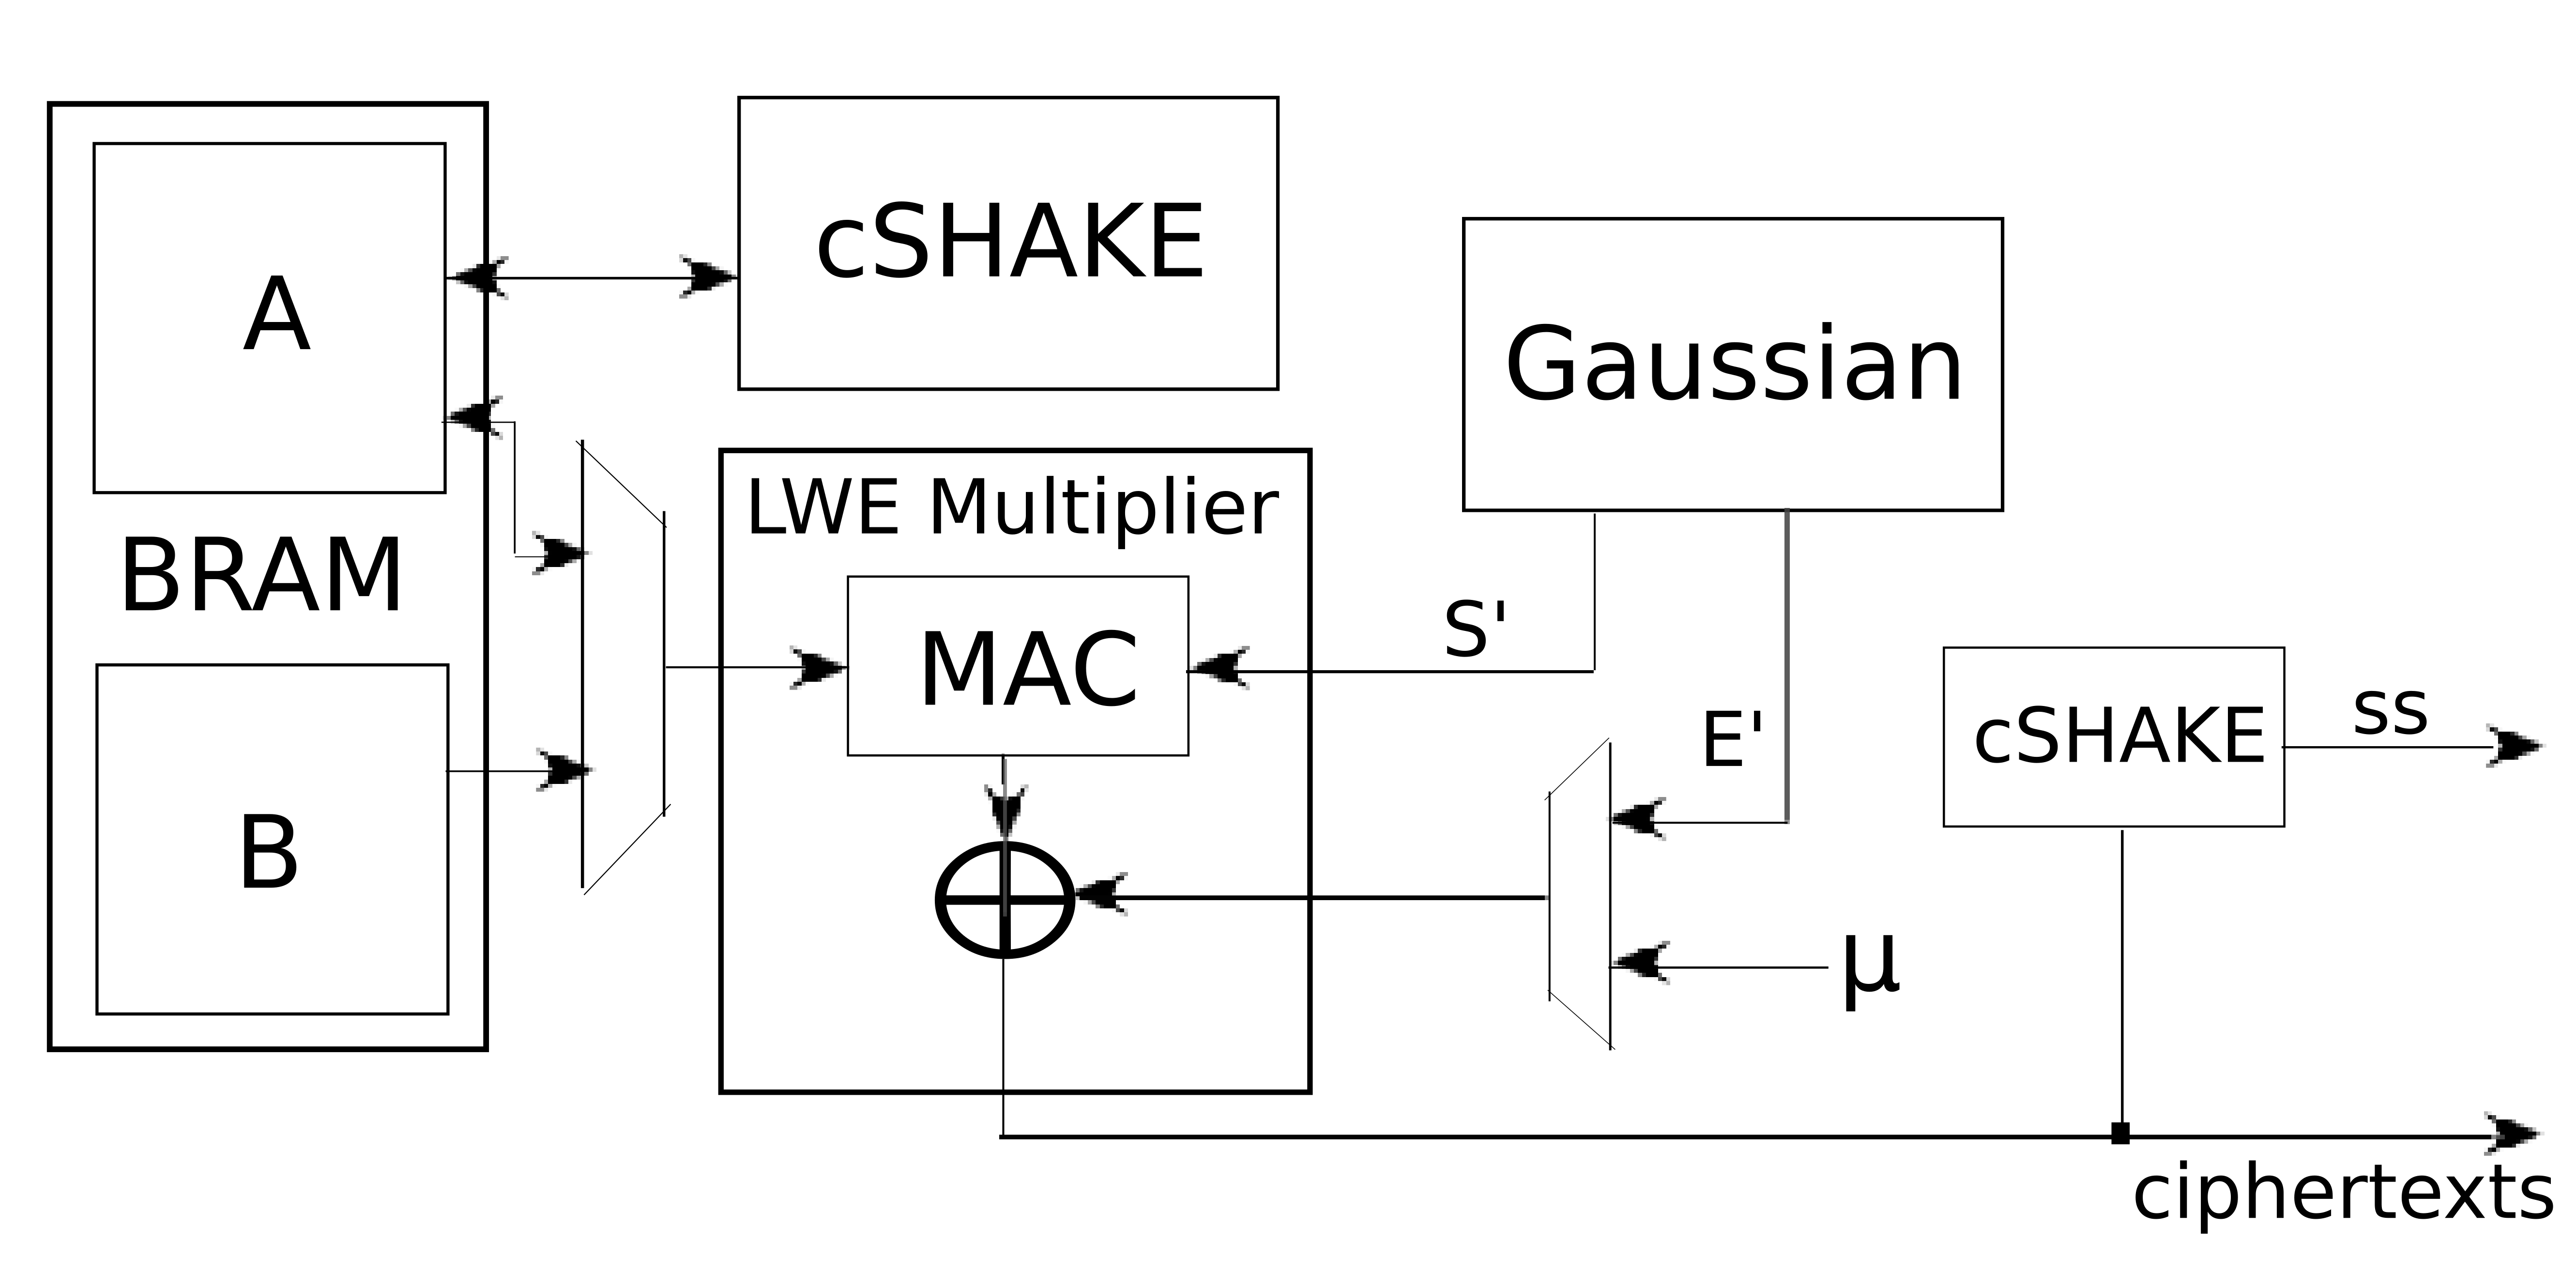
\includegraphics[width=0.95\textwidth,]{figures/FPGA_encaps.png}
  	\caption{A high-level architecture of the FPGA design of \textsf{FrodoKEM-cSHAKE} Encaps.}
  	\label{fig:fpga}
  \end{figure}

\subsection{Additional Modules}

The generation of the deterministic matrix $\mathbf{A}$ uses cSHAKE. For the cSHAKE implementation, a balanced design is used which is based around the mid-range core of KECCAK\footnote{See \url{https://keccak.team/2012/mid_range_hw.html} for more information on the core.}. Due to the deterministic nature of the matrix $\mathbf{A}$, it does not need to be stored in its entirety. This is essential, as otherwise the storage requirements would exceed the capacity of the FPGA, even for the smaller parameter set. Instead, enough of the matrix is pre-generated during the initialization stage, where the remaining matrix is generated on-the-fly, which continuously reuses the same memory blocks. This is similar to the page-flip technique used for $\mathbf{S}^\prime$. This module runs in parallel to the LWE multiplication core and is thus not apart of the critical path and the clock cycle counts of the operations. 

Error sampling is another important module within \textsf{FrodoKEM}. Both \textsf{FrodoKEM-640} and \textsf{FrodoKEM-976} parameter sets require a slightly different distribution, however the standard deviations are close enough to essentially utilize the same FPGA area and performance. A large number of samples are required during a run of \textsf{FrodoKEM}, due to this a fast but rather large sampler is designed in order to keep up with the LWE multiplier. Instead of using a binary search for the table look-up, a large number of comparators are used in order to instantly output an error distribution value in the look-up table.

%This architecture is somewhat shared for Decaps which requires more BRAM storage.

%Most of the remaining operations in Frodo, such as packing, unpacking, modular reduction, encoding, and decoding, happen for free or in cheap parallel processes. The packing process happens naturally d

%Modular reduction is for free!

%Gaussian sampler uses a fast design...
\section{Microcontroller Design}

We present four implementations of \textsf{FrodoKEM}. We implemented both parameter sets \textsf{FrodoKEM-640} and \textsf{FrodoKEM-976}
and we also implemented both possible pseudo-random numbers generators for the generation of $\mathbf{A}$. For AES, we rely on the optimized implementation by Schwabe and Stoffelen \cite{DBLP:conf/sacrypt/SchwabeS16} and for cSHAKE we use the assembly implementation from the official KECCAK code package \cite{bertoni2016keccak}.

\subsection{Target Platform}

We evaluate our microcontroller implementation of \textsf{FrodoKEM} on the STM32F407 Discovery board that has a 32-bit ARM Cortex-M4F microprocessor that runs with up to 168 MHz. Our development board comes with 192 kilobyte of RAM and one megabyte of Flash memory. Furthermore the Cortex-M4 features powerful DSP instructions like single-cycle multiply-with-accumulate and a true random number generator based on analog noise. However, in contrast to other M4-based microcontrollers, our development board does not have an AES-accelerator that could be used to speed-up \textsf{FrodoKEM-AES}. As development environment we use CooCox CoIDE version 1.7.7 with gcc-arm-none-eabi 5.4 2016 toolchain. The Cortex-M4F has 13 general purpose registers and ($R0-R12$), one register reserved for the stack pointer, a link register, one register reserved for the program counter, and special-purpose program status registers. When mixing C with assembly it is important to note that the calling convention requires parameters to be in $R0-R3$ and the result to be in $R0-R1$. The link register can be used as general purpose register as well, if the assembly function does not call any other function and its original value is restored before leaving the function.

\subsection{High-level Memory Optimization}

The official specification of \textsf{FrodoKEM} reports a peak stack memory usage of 189,176 bytes for \textsf{FrodoKEM-976-AES}. As our microcontroller has only access to 192 kilobytes of RAM, we carefully analyze the memory allocation of the reference implementation to see whether we can make the implementation more efficient in terms of memory usage. Keep in mind that for many applications there is another software running beside the KEM, therefore it is sensible to reduce the memory consumption as much as possible without sacrificing performance. With the help of the flow chart of the most important operations in \textsf{FrodoKEM} (Figure \ref{fig:flowchart_encaps} and \ref{fig:flowchart_decaps}), it is easily possible to see which matrices are used for which computations. The highlighted intermediate values are large arrays with $n \times \bar{n}$ elements. As we store each element in two bytes, this means that one large array requires $976 \times 8 \times 2 = 15,616$ bytes of RAM for each large array for \textsf{FrodoKEM-976-AES}. The non-highlighted intermediate values are small ($\bar{n} \times \bar{n}$ elements, i.e. 128 bytes) and therefore we focus on optimizing the large ones. 

The first thing to note about decapsulation, as shown in Figure \ref{fig:flowchart_decaps}, is that we need memory for at least two large arrays. For instance, during the computation of $\mathbf{B}''$, both inputs $\mathbf{E'}$ and $\mathbf{S'}$ are large. While $\mathbf{E'}$ can be generated on the fly, $\mathbf{S'}$ is loaded multiple times during the multiplication by $\mathbf{A}$ and therefore on-the-fly computation would imply regenerating the same value over and over again. Therefore we decided that the better trade-off would be to keep storage space for at least two large arrays. Another thing to note is that the right-hand side can be computed completely independent from the left-hand side. Therefore we can store $\mathbf{S'}$ in one of our two memory slots for large arrays and compute $\mathbf{V}$ and $\mathbf{B''}$ using the other memory slot. Once $\mathbf{V}$ and $\mathbf{B''}$ are calculated, $\mathbf{S'}$ is no longer used and can be replaced by $\mathbf{B'}$.

In the flow chart of encapsulation in Figure \ref{fig:flowchart_encaps} we can see that two large arrays are also sufficient for the encapsulation as the sampling of $\mathbf{E'}$ and the unpacking of $\mathbf{B}$ can be done on-the-fly. In fact the encapsulation needs even less memory as for instance the packing of $\mathbf{B'}$ could be done on-the-fly as well. But as the bottleneck in terms of memory consumption is the decapsulation, we do not further optimize the encapsulation.

\begin{figure*}[tbhp]
\centering

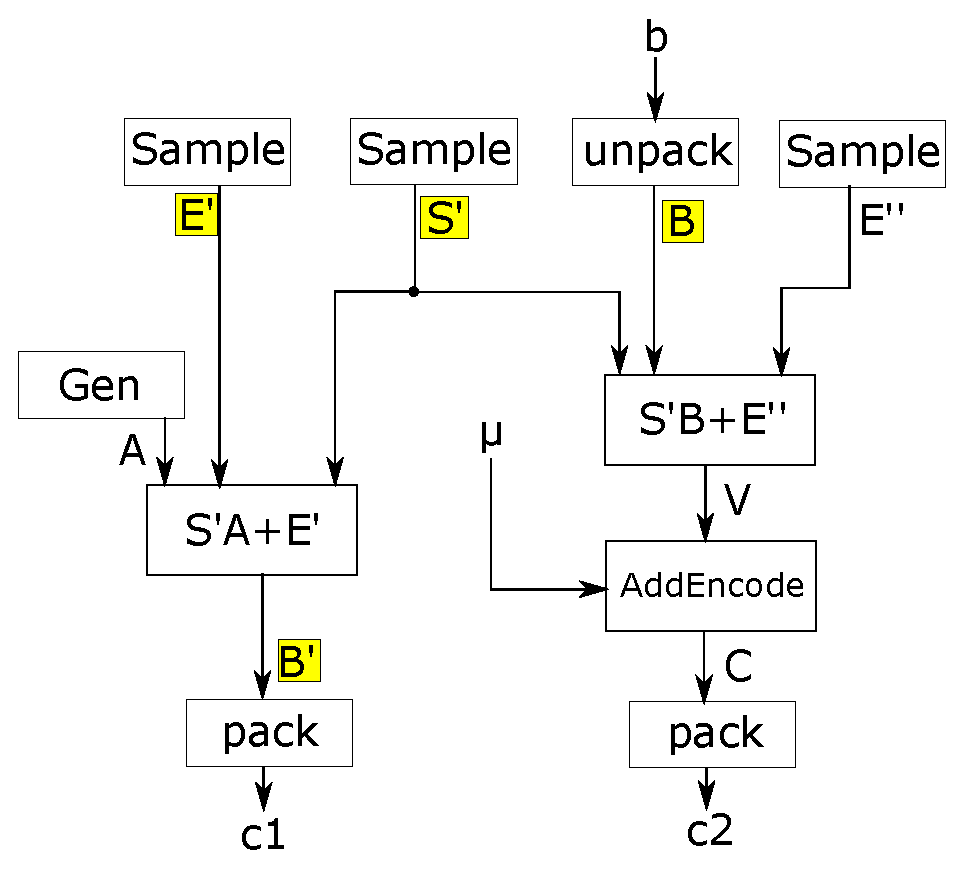
\includegraphics[scale=0.6]{figures/frodo_flowchart_encaps}

\caption{Flowchart of the encapsulation. Yellow highlighted matrices are $n \times \bar{n}$ matrices.}
\label{fig:flowchart_encaps}
\end{figure*}

\begin{figure*}[tbhp]
\centering

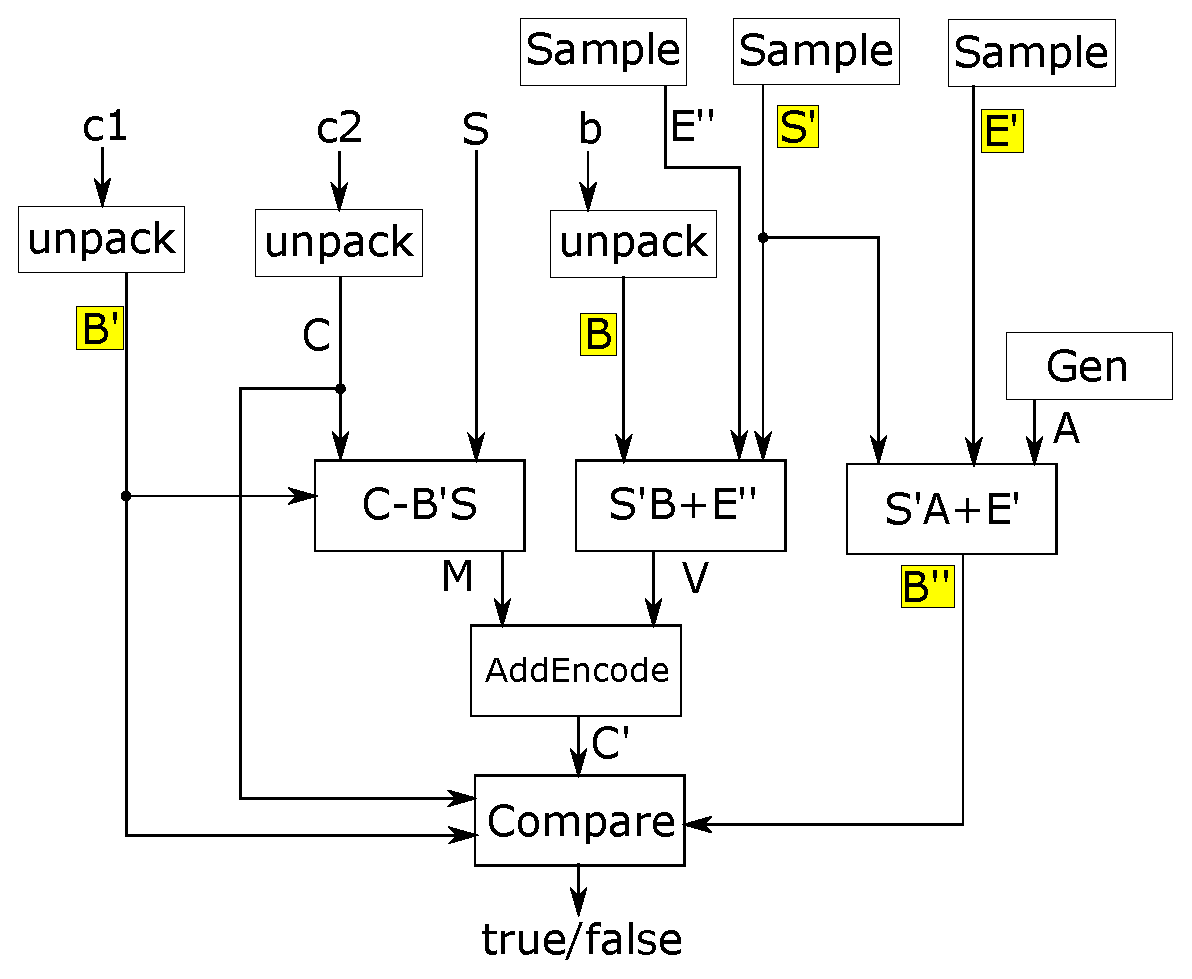
\includegraphics[scale=0.6]{figures/frodo_flowchart_decaps}

\caption{Flowchart of the decapsulation. Yellow highlighted matrices are $n \times \bar{n}$ matrices.}
\label{fig:flowchart_decaps}
\end{figure*}

\subsection{Low-level Assembly Optimization}

Our measurements indicate that besides the generation of the matrix $\mathbf{A}$, the multiplication of $\mathbf{A}$ with the secret matrix consumes most of the cycles, and therefore optimizing the multiplication is profitable. The simple operation of multiplication consumes just a small part of the cycles, the loading and storing of the matrix entries is the decisive part. Therefore minimizing the memory accesses is the key to a short run-time. Since the generation of the matrix $\mathbf{A}$ needs to be computed on-the-fly due to the memory constraints on the ARM Cortex-M4F, the multiplication cannot be done on the whole matrix $\mathbf{A}$ at once. We chose to generate $\mathbf{A}$ row-by-row when computing $\mathbf{AS}$. For the computation of $\mathbf{S'A}$ the generation of $\mathbf{A}$ depends on the choice of the permutation function. Writing the multiplication in assembly language gives us more control over the implementation and allows us to incorporate enhancements the compiler cannot engineer. Since the amount of memory accesses is substantial for the speed, our goal is to load the necessary matrix entries from RAM as rarely as possible and use all the available registers.

When $\mathbf{A}$ is generated on-the-fly, a straightforward implementation of the multiplication of $\mathbf{AS}$ has two loops. The first loop iterates over the columns of $\mathbf{S}$ with $\bar{n}$ iterations. The second loop iterates over the rows of $\mathbf{S}$, respectively the entries of the generated row of $\mathbf{A}$ with $n$ iterations.  But as $\bar{n} = 8$ in both parameter sets, it is possible to implement the matrix multiplication by using only one loop. During the multiplication of one row of $\mathbf{A}$ with $\mathbf{S}$, only eight entries of $\mathbf{AS}$ are computed. Since these entries are the sum of the products of $n$ multiplications, they are often updated during the computation. Storing the eight entries of $\mathbf{AS}$ in registers during the whole computation enables us to save many memory accesses: instead of iterating over the eight columns of $\mathbf{S}$, it is possible to process one entry of $\mathbf{A}$ with a complete row from $\mathbf{S}$ during one iteration. Figure \ref{fig:mul} presents this concept graphically.

  \begin{figure}[tbhp]
  	\centering
  	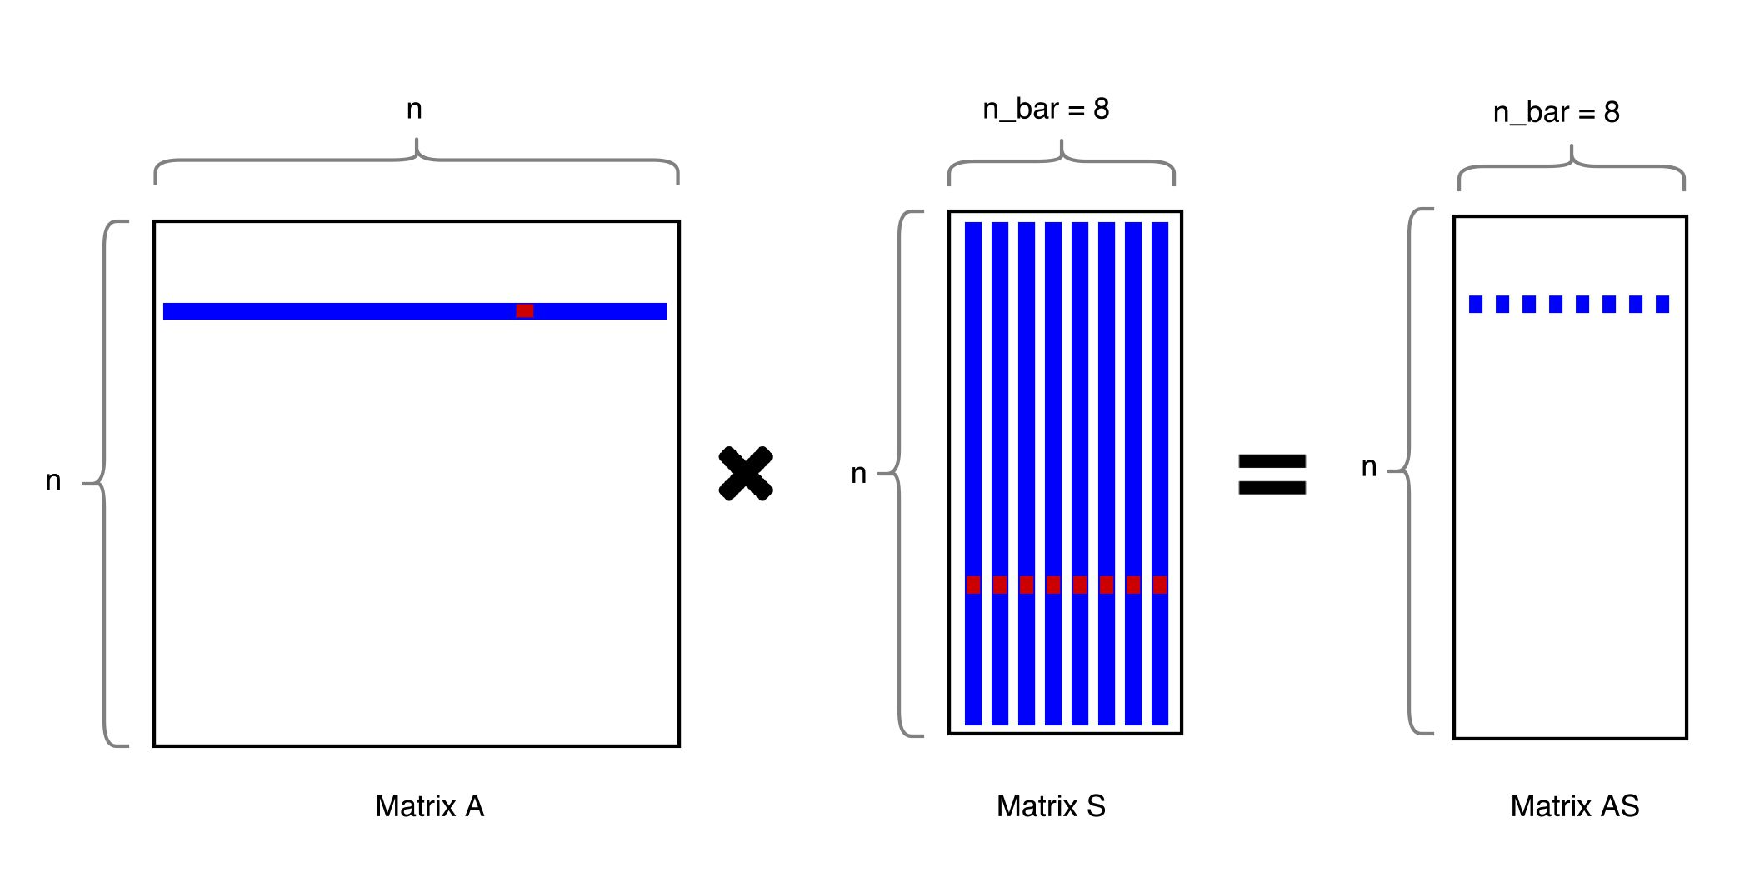
\includegraphics[width=1\textwidth,]{figures/mul.pdf}
  	\caption{Concept of the multiplication of one row of $\mathbf{A}$ with $\mathbf{S}$ effectively. Blue entries are affected by one function call, red entries are loaded during one iteration.}
  	\label{fig:mul}
  \end{figure}

The multiplication of $\mathbf{A}$ and matrix $\mathbf{S'}$ is slightly different, and variates with the use of either AES or cSHAKE. With cSHAKE, the matrix $\mathbf{A}$ is intended to be generated only in entire rows, which is convenient for the computation of $\mathbf{AS}$, but inefficient for the computation of $\mathbf{S'A}$, because one row of $\mathbf{A}$ affects all elements of $\mathbf{S'A}$. 
With AES, $\mathbf{A}$ is generated in blocks of 128 bits, therefore it is not only possible to generate $\mathbf{A}$ row-by-row but also by producing eight columns at a time. In a straightforward implementation, this leads to a third  loop iterating over the eight columns. The fact that the number of processed columns of $\mathbf{A}$ is eight, just as the parameter $\bar{n}$, enables us to use the same concept that we used for the multiplication of $\mathbf{S'A}$. We illustrate this concept in Figure \ref{fig:mulcol}. To avoid nested loops, we unroll the loop that gets added due to the eight columns. We end up with eight loops that are run through \emph{after} each other.
	
 \begin{figure}[tbhp]
   	\centering
   	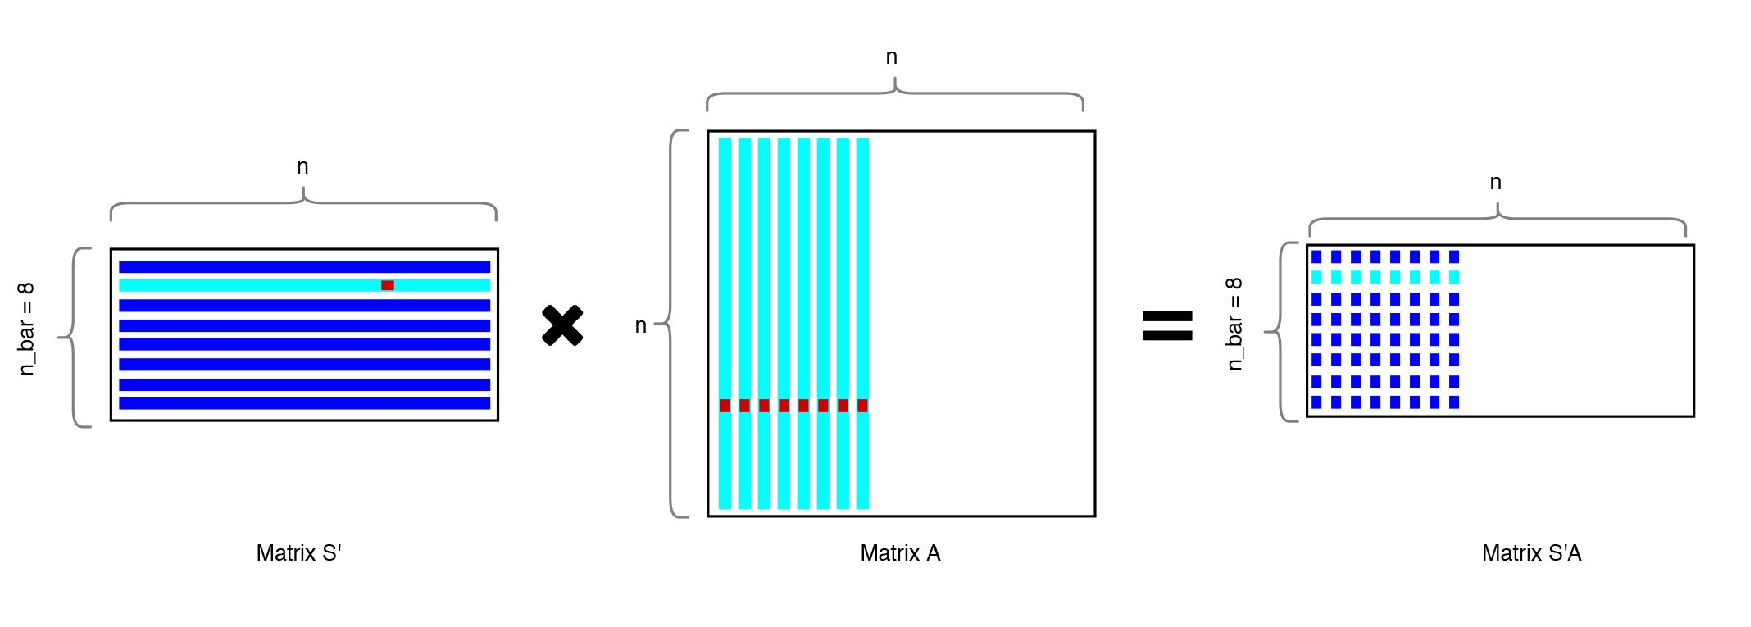
\includegraphics[width=1\textwidth,]{figures/colmul.pdf}
   	\caption{Concept of the multiplication of 8 columns of $\mathbf{A}$ with $\mathbf{S'}$ effectively. Blue and light blue entries are affected by one function call, light blue entries are loaded by one entire loop, red entries are loaded during one iteration.}
   	\label{fig:mulcol}
 \end{figure}

The ARM Cortex-M4F offers 13 general purpose registers $R0-R12$ which we use all in our assembly matrix multiplication to maximize memory efficiency. Furthermore we use the designated link register $R14$ whose content we preserve on the stack. In $R0$ a pointer to matrix $\mathbf{A}$ is passed, in $R1$ a pointer to matrix $\mathbf{S}$, and in $R2$ a pointer to matrix $\mathbf{B}$. After loading the eight relevant entries of $\mathbf{B}$ into the registers $R4-R11$, we use $R2$ to store elements of $\mathbf{A}$. In $R3$ we pass the parameter $n$, which defines the number of iterations through the loop. In $R12$ and $R14$ entries of $\mathbf{S}$ are stored.

In both parameter sets, entries of matrices are stored in 16-bit data types, but the ARM Cortex-M4F is a 32-bit architecture. This enables us to reduce memory access, by loading two entries of matrix $\mathbf{A}$ simultaneously, as in Line 1 of Listing \ref{lst:loop1}. In the next line we use an instruction to load multiple aligned words, to get four entries of $\mathbf{S}$ by only one instruction. The single-cycle multiply-with-accumulate capabilities are very valuable for the actual matrix multiplication, used for example in Line 3 of Listing \ref{lst:loop1}.

\begin{lstlisting}[caption={Multiplication in Assembly}\label{lst:loop1}]
ldr r2, [r0], #4     //r2=a_ij+1, a_ij
ldmia r1!, {r12,r14} //r12=s_ij+1, s_ij, r14=s_ij+3,s_ij+2
mla r4, r2, r12, r4  //r4=r2*r12+r4
lsr r12, r12, #16    //r12=s_ij+1
mla r5, r2, r12, r5
mla r6, r2, r14, r6
lsr r14, r14, #16
mla r7, r2, r14, r7
\end{lstlisting}

\subsection{Protection Against Timing Side Channels}
Our implementations using cSHAKE have a constant timing and are therefore protected against timing attacks. The AES implementation from \cite{DBLP:conf/sacrypt/SchwabeS16} is very efficient but due to the caches on our development board not timing-constant. Therefore we disabled the data and instruction cache by clearing bit 9 and bit 10 of the \texttt{FLASH\_ACR} register. We noticed only a negligible drop in performance ($< 1$\%) after disabling the caches.

\section{Results and Comparison}
In this section we discuss the results of our FPGA and microcontroller implementations and compare our implementations with others. In particular, we also compare with implementations of \textsf{NewHopeUSENIX}, even though comparing a standard lattice-based scheme with an ideal lattice-based scheme is not exactly an apples-to-apples comparison (as discussed in Section \ref{sec:ringvsstandard}). Our intention behind this comparison is to show the cost of removing the potential additional attack vector of ideal lattices (i.e., the ring structure).
\subsection{FPGA Results}

%\begin{table}[tbhp]
%\caption{Resource consumption of \textsf{FrodoKEM-cSHAKE} on a Xilinx Artix-7 XC7A35T FPGA.}
%\label{tab:res_fpga}
%\begin{center}
%\begin{tabular}{|c|c|c|c|c|c|c|}
%\hline
%%& \multicolumn{2}{c|}{\textsf{FrodoKEM-AES}} &\multicolumn{2}{c|}{\textsf{FrodoKEM-cSHAKE}} &&\\
%\textsf{FrodoKEM} Operation	& LUT/FF & Slice & DSP & BRAM & MHz & Ops/sec\\
%\hline
%\textsf{FrodoKEM-640} Keypair	& 6621/3511 & 1845 & 1 & 6 & 167 & 51 \\
%\textsf{FrodoKEM-640} Encaps	& 6745/3528 & 1855 & 1 & 11 & 167 & 51 \\
%\textsf{FrodoKEM-640} Decaps	& 7220/3549  & 1992  & 1 & 16 & 162 & 49 \\ \hline
%\textsf{FrodoKEM-976} Keypair	& 7155/3528 & 1981 & 1 & 8 & 167 & 22 \\
%\textsf{FrodoKEM-976} Encaps	& 7209/3537 & 1985 & 1 & 16 & 167 & 22 \\
%\textsf{FrodoKEM-976} Decaps	& 7773/3559 & 2158 & 1 & 24 & 162 & 21 \\ %\hline\hline
%%\textsf{NewHope-1024} Server \cite{oder2017implementing}	& 5142/4452 & - & 2 & 4 & 125 & 731 \\
%%\textsf{NewHope-1024} Client \cite{oder2017implementing}	& 4498/4635 & - & 2 & 4 & 117 & 653 \\ \hline
%%\textsf{LWE} Encryption \cite{HoweMORGB16_1} & 6078/4676 & 1811 & 1 & 73 & 125 & 1272 \\
%\hline
%\end{tabular}
%\end{center}
%\end{table}

Table \ref{tab:comp_fpga} provides post-place and route results of the proposed hardware designs, as well as comparative lattice-based cryptographic hardware designs. The 18Kb BRAM usage follows the requirements of the inputs of the operations, those being the public-key, the secret-key, and the ciphertext information. The increased of BRAM usage in Decaps results in a slight decrease in clock frequency. The area consumption of all the modules are similar, at least for each parameter set. This is essentially due to the reuse of the LWE multiplication core, which is reused for all vector-matrix multiplication and error addition operations. The increase between parameter sets is due to an increase from 640 to 976 in the matrix dimension, the rest of the design essentially remains the same.


\begin{table}[tbhp]
\caption{FPGA resource consumption of the proposed \textsf{FrodoKEM-cSHAKE} hardware design, with its sub-modules ($^*$), alongside \textsf{NewHopeUSENIX-1024} \cite{oder2017implementing} and \textsf{Standard-LWE} encryption \cite{DBLP:conf/dac/HoweMORGB16} hardware designs for comparison. \textsf{FrodoKEM} and \textsf{NewHopeUSENIX-1024} utilize a Xilinx Artix-7 FPGA and \textsf{Standard-LWE} utilizes a Xilinx Spartan-6 FPGA.}
\label{tab:comp_fpga}
\begin{center}
\resizebox{\textwidth}{!}{
\noindent\makebox[\textwidth]{
\begin{tabular}{|c|c|c|c|c|c|c|}
\hline
%& \multicolumn{2}{c|}{\textsf{FrodoKEM-AES}} &\multicolumn{2}{c|}{\textsf{FrodoKEM-cSHAKE}} &&\\
Cryptographic Operation	& LUT/FF & Slice & DSP & BRAM & MHz & Ops/sec\\
\hline
\textsf{FrodoKEM-640} Keypair 	& 6621/3511 & 1845 & 1 & 6 & 167 & 51 \\
\textsf{FrodoKEM-640} Encaps	& 6745/3528 & 1855 & 1 & 11 & 167 & 51 \\
\textsf{FrodoKEM-640} Decaps	& 7220/3549  & 1992  & 1 & 16 & 162 & 49 \\ \hline
\textsf{FrodoKEM-976} Keypair	& 7155/3528 & 1981 & 1 & 8 & 167 & 22 \\
\textsf{FrodoKEM-976} Encaps	& 7209/3537 & 1985 & 1 & 16 & 167 & 22 \\
\textsf{FrodoKEM-976} Decaps	& 7773/3559 & 2158 & 1 & 24 & 162 & 21 \\ \hline
cSHAKE$^*$	& 2744/1685 & 766 & 0 & 0 & 172 & 1.2m \\
Error+AES Sampler$^*$ & 1901/1140 & 756 & 0 & 0 & 184 & 184m \\

\hline\hline
\textsf{NewHopeUSENIX} Server \cite{oder2017implementing} 	& 5142/4452 & 1708 & 2 & 4 & 125 & 731 \\
\textsf{NewHopeUSENIX} Client \cite{oder2017implementing}	& 4498/4635 & 1483 & 2 & 4 & 117 & 653 \\ \hline
\textsf{LWE} Encryption \cite{DBLP:conf/dac/HoweMORGB16}  & 6078/4676 & 1811 & 1 & 73 & 125 & 1272 \\
\hline
\end{tabular}}}
\end{center}
\end{table}

Hardware results are also provided for the main components required; the error distribution sampler and the cSHAKE module. As per the specifications, the error sampler is combined with AES as a PRNG input to the lookup table. The large area consumption of this module is due to the use of AES, as well as employing a large number of comparators in order for high throughput. One cSHAKE module is used for generating the randomness for the matrix $\mathbf{A}$ and a second is used to generate the shared secret $\mathbf{ss}$ on-the-fly, which makes these cSHAKE modules the largest overall. The remaining area usage is consumed by control logic and the LWE multiplier; which requires a DSP for multiplication and a reasonable amount of LUTs for storage.


In Table \ref{tab:clks_fpga} we present the cycle counts for our FPGA designs. Clock cycle counts in Table \ref{tab:clks_fpga} are equivalent for the PRNG choice (either AES or cSHAKE) as this module runs in parallel to the vector-matrix multiplication within the LWE multiplication core, and does not affect the critical path of the operations (as described in Section \ref{sec:lwe_core}). The clock cycle counts for each cryptographic operation are defined by the MAC operations of all the matrix-matrix multiplications they require. Moreover, the multiplication of the largest matrices in each cryptographic operation, that is; $\mathbf{B} \leftarrow \mathbf{A} \mathbf{S} + \mathbf{E}$ for key generation, $\mathbf{B}^\prime \leftarrow \mathbf{S}^\prime \mathbf{A} + \mathbf{E}^\prime$ for encapsulation, or $\mathbf{B}^{\prime\prime} \leftarrow \mathbf{S}^\prime \mathbf{A} + \mathbf{E}^\prime$ for decapsulation, respectively contribute 100\%, 97.5\%, and 97.5\% to their overall clock cycle counts. As described in Section \ref{sec:frodo_fpga}, there is a one-time initialisation stage, for loading input information, initialising modules, and pre-storage matrices. This process lasts between 5.1k and 23.5k clock cycles, depending on the operation and parameter set used. This extra latency is not included in Table \ref{tab:clks_fpga} as it is negligible, even for one run of a \textsf{FrodoKEM} operation (at most, $< 0.5 \%$), and becomes even more so when averaged over numerous operations.

%For example in \textsf{FrodoKEM-640} encaps, this stage requires 5.1k clock cycles to load key information

\begin{table}[tbhp]
\caption{Clock cycle counts for our FPGA implementations of \textsf{FrodoKEM}.}
\label{tab:clks_fpga}
\begin{center}
\begin{tabular}{|l|r|r|r|r|}
\hline
& \multicolumn{2}{c|}{\textsf{FrodoKEM-AES}} &\multicolumn{2}{c|}{\textsf{FrodoKEM-cSHAKE}} \\
Operation	  & $n=640$ & $n=976$ & $n=640$ & $n=976$\\
\hline
%Operation 1					& xxx & xxx & xxx & xxx \\
%Operation 2					& xxx & xxx & xxx & xxx \\
%Operation 3					& xxx & xxx & xxx & xxx \\
Keypair							& 3,276,800 & 7,620,608 & 3,276,800 & 7,620,608 \\
Encaps							& 3,317,760 & 7,683,072 & 3,317,760 & 7,683,072 \\
Decaps							& 3,358,720 & 7,745,536 & 3,358,720 & 7,745,536 \\
\hline
\end{tabular}
\end{center}
\end{table}

Comparison results for related works is given in Table \ref{tab:comp_fpga}. The FPGA device used, the Xilinx Artix-7 XC7A35T FPGA, is similar to the one used by Oder and G{\"u}neysu \cite{oder2017implementing}, in order for a fair comparison. Although the \textsf{NewHopeUSENIX} design outperforms our proposed designs in terms of operations per second, the area consumption is comparable. The loss in throughput is expected and almost entirely due to the number of clock cycles required for each operation; \textsf{NewHopeUSENIX} requires 171k clock cycles for the server-side operations whereas \textsf{FrodoKEM} requires 3.3m. The increase in memory requirements is due to the differences in the key sizes, since \textsf{NewHopeUSENIX} uses polynomials instead of the matrices used in \textsf{FrodoKEM} (as mentioned in Section \ref{sec:ringvsstandard}).

The only other implementation of standard lattice-based cryptography in hardware is by Howe et al. \cite{DBLP:conf/dac/HoweMORGB16}, referred to as \textsf{Standard-LWE}, and is discussed here for comparison. The area consumptions are similar due to the similar LWE multiplication operations required, however, Howe et al. uses significantly smaller matrix dimensions in comparison to the \textsf{FrodoKEM} parameters, and hence we see an improvement. Moreover, their use of BRAM is significantly larger, due to precomputed keys, which we mitigate by using on-the-fly generation. Reusing keys is discussed by the authors of \textsf{FrodoKEM} \cite[Sec. 5.1.4]{frodo-nist} but is not recommended due to the potential attack vector it provides. Additionally, we also wanted to keep the memory requirements low and therefore decided to not store the entire matrix $\mathbf{A}$ in memory. The throughput performance of \textsf{Standard-LWE} is much higher in comparison to our research, due to a much lower clock cycle count of 98k required. This is essentially due to, again, the significantly smaller matrix dimensions and hence less multiplications required. Comparing the overall security targets of the schemes shows that the \textsf{Standard-LWE} implementation only provides 128 bits of \textit{classical} security, whereas our implementations provide 128 and 192 bits of post-quantum security.

%\textsf{Stanard-LWE} achieves such a low clock cycle count because the matrix $\mathbf{A}$ is precomputed and stored in memory, whereas in our implementation $\mathbf{A}$ is generated on-the-fly and clearly the bottleneck. 



\subsection{Microcontroller Results}
We use the pqm4 framework \cite{pqm4} to evaluate the proposed microcontroller implementation. In the framework, the running time of an operation is measured in cycle counts using libopencm3\footnote{\url{http://libopencm3.org/}}. The framework can also measure the stack usage with the help of stack canaries. Our development board runs at a clock frequency of 168 MHz.

In Table \ref{tab:res_micro} we show the cycle counts for the major building blocks of \textsf{FrodoKEM} as well as the entire key pair generation, encapsulation, and decapsulation. At 168 MHz, the key generation takes 266 ms, the encapsulation takes 284 ms, and the decapsulation takes 286 ms for \textsf{FrodoKEM-640-AES}. For \textsf{FrodoKEM-940-AES} the cycle counts are more than twice as high as for \textsf{FrodoKEM-640-AES}. The main reason for that is that the size of the matrix $\mathbf{A}$ grows quadratically when $n$ grows and the generation of $\mathbf{A}$ is the most time consuming part of our implementation. Further speed-ups could be achieved by speeding up the AES implementation. However, to the best of our knowledge, the implementation by Schwabe and Stoffelen \cite{DBLP:conf/sacrypt/SchwabeS16} that we used in our implementation is already the fastest published AES implementation. Some Cortex-M4-based microcontrollers also have access to an on-board hardware AES engine that would further speed up the AES. The implementations of \textsf{FrodoKEM-cSHAKE} are slower than \textsf{FrodoKEM-AES} implementations as cSHAKE is based on KECCAK and hardware platforms are where KECCAK really excels on, not software \cite{SHA3}. Therefore we expected \textsf{FrodoKEM-cSHAKE} to have a worse performance than \textsf{FrodoKEM-AES}.  

We furthermore see in Table \ref{tab:res_micro} that the $\mathbf{AS} + \mathbf{E}$ is the most time consuming part of the key pair generation as it accounts for 93\% of the run time for \textsf{FrodoKEM-640-AES}. Similarly $\mathbf{S}^\prime \mathbf{A} + \mathbf{E}^\prime$ is bottleneck for encapsulation and decapsulation (88\% resp. 87\%). The second most time-consuming operation is the sampling of a noise matrix. We measured the performance of noise sampling for matrices with dimension $n \times \bar{n}$. This operation is performed twice during every run of key pair generation, encapsulation, and decapsulation. It accounts for 6\% of the run time of each of the three algorithms (\textsf{FrodoKEM-640-AES}). In comparison to the computation of $\mathbf{AS} + \mathbf{E}$ or $\mathbf{S}^\prime \mathbf{A} + \mathbf{E}^\prime$, multiplications of smaller matrices cost much less cycles, as one can see in the cycle counts for $\mathbf{S}^\prime \mathbf{B} + \mathbf{E}^{\prime\prime}$.

\begin{table}[tbhp]
\caption{Cycle counts for our microcontroller implementation measured at a clock frequency of 168 Mhz.}
\label{tab:res_micro}
\begin{center}
\begin{tabular}{|l|r|r|r|r|}
\hline
& \multicolumn{2}{c|}{\textsf{FrodoKEM-AES}} &\multicolumn{2}{c|}{\textsf{FrodoKEM-cSHAKE}} \\
Operation	  & $n=640$ & $n=976$ & $n=640$ & $n=976$\\
\hline
$\mathbf{S}^\prime \mathbf{B} + \mathbf{E}^{\prime\prime}$	& 451,442  		& 687,728  		& 451,442  		& 687,728  \\
$\text{SampleMatrix}(\cdot,n,\bar{n},\cdot,\cdot)$					& 1,344,962  	& 1,480,483  	& 1,344,963  	& 1,480,484  \\
$\mathbf{AS} + \mathbf{E}$																	& 41,308,745 	& 96,035,515  & 82,256,529  & 181,809,613  \\
$\mathbf{S}^\prime \mathbf{A} + \mathbf{E}^\prime$					& 41,833,535  & 97,266,270  & 106,178,196 & 244,078,721  \\\hline
Keypair							& 44,603,160   & 101,273,066  & 85,585,315 & 187,070,653  \\
Encaps							& 47,742,966   & 106,933,956  & 112,103,350  & 253,735,550  \\
Decaps							& 48,051,929   & 107,393,295  & 112,442,770   & 254,194,895  \\
\hline
\end{tabular}
\end{center}
\end{table}

In Table \ref{tab:res_micro_mem} we list the peak stack usage for our implementations. For $n = 976$ the \textsf{FrodoKEM} specification \cite{frodo-nist} reports a peak stack memory usage of 189 kilobytes when using AES as PRNG and 156 kilobytes when using cSHAKE. The specification reports at most 81,836 bytes as static library size for non-vectorized implementations. As our development board has access to 192 kilobytes of RAM and one megabyte of Flash memory, the peak stack usage is what we focus on in the following. We managed to reduce these numbers so that the implementation comfortably fits onto the microcontroller and still leaves space for other applications running on it. For the AES-based implementation we reduced the memory consumption by 66\% and for the cSHAKE implementation we reduced it by 63\%.

\begin{table}[tbhp]
\caption{Stack usage in bytes for our microcontroller implementation.}
\label{tab:res_micro_mem}
\begin{center}
\begin{tabular}{|l|r|r|r|r|}
\hline
& \multicolumn{2}{c|}{\textsf{FrodoKEM-AES}} &\multicolumn{2}{c|}{\textsf{FrodoKEM-cSHAKE}} \\
Operation	  & $n=640$ & $n=976$ & $n=640$ & $n=976$\\
\hline
Keypair							& 23,396   & 35,484  & 22,376  & 33,800   \\
Encaps							& 41,292   & 63,484  & 37,792  & 57,968   \\
Decaps							& 51,684   & 63,628  & 48,184  & 58,112   \\
\hline
\end{tabular}
\end{center}
\end{table}


\begin{table}[tbhp]
\begin{center}
\caption{Comparison of our microcontroller implementation with other implementations.}
\label{tab:micro_comparison}
\begin{tabular}{|l|l|r|r|}
\hline
Implementation & Platform & Security Level & Cycle counts\\\hline
\textsf{FrodoKEM-976-AES} (\textbf{this work})	& Cortex-M4 & 192 bits  & 315,600,317\\
\textsf{FrodoKEM-640-cSHAKE} \cite{pqm4} & Cortex-M4 & 128 bits & 318,037,129 \\
\textsf{KyberNIST-768} \cite{pqm4} & Cortex-M4 & 192 bits & 4,224,704 \\
\textsf{NewHopeUSENIX-1024} \cite{alkim2016newhope}	& Cortex-M4 &255 bits & 2,561,438 \\
ECDH scalar multiplication \cite{DBLP:journals/dcc/DullHHHPSS15} &  Cortex-M0 & pre-quantum & 3,589,850\\
\hline
\end{tabular}
\end{center}
%\vspace{-0.7cm}
\end{table}

In Table \ref{tab:micro_comparison} we compare our implementation with other implementations of key exchange schemes on Cortex-M microprocessors. Our implementation of \textsf{FrodoKEM-976-AES} has a similar performance compared to the implementation of \textsf{FrodoKEM-640-cSHAKE} from the pqm4 library \cite{pqm4} even though the security level is higher (192 vs. 128 bits). Our implementation is two orders of magnitude slower than the \textsf{NewHopeUSENIX} implementation from \cite{alkim2016newhope}. The reason for that is that \textsf{NewHopeUSENIX} is based on ideal lattices that are inherently much more efficient as the main operation in ideal lattice-based cryptography is polynomial multiplication. Polynomial multiplication in integer rings can be efficiently realized with the number-theoretic transform that has a complexity of $O(n \log (n))$ while the matrix operations in \textsf{FrodoKEM} have a complexity of $O(n^2)$. Therefore a decently optimized implementation of a scheme based on ideal lattices will always be faster than any implementation of a scheme based on standard lattices targeting a similar security level. Furthermore, the implementation in \cite{alkim2016newhope} is only secure against chosen-plaintext attackers, not chosen-ciphertext attackers. Unsurprisingly the \textsf{KyberNIST-768} implementation from pqm4 also provides a better performance, as \textsf{KyberNIST-768} is a module lattice-based scheme that still retains some of the structure of ideal lattices and in particular also benefits from the speed-ups from the number-theoretic transform. The ECDH implementation of \cite{DBLP:journals/dcc/DullHHHPSS15} is also much more efficient. But as ECDH is not secure against attacks by quantum computers, it cannot be considered as alternative to \textsf{FrodoKEM}.

While being significantly slower than implementations of other schemes, \textsf{FrodoKEM} is also a very conservative choice that does not suffer from relying on a structured lattice as potential additional attack vector (like for instance \textsf{NewHopeUSENIX} does). Depending on the use case it might be sensible to use \textsf{NewHopeUSENIX} in scenarios that demand high efficiency and moderate security and use \textsf{FrodoKEM} in cases that have very high security requirements.
\section{Conclusion}
In this paper we present a thorough evaluation of the NIST post-quantum standardization candidate \textsf{FrodoKEM}  on embedded devices. We have developed an FPGA implementation that fits into 2000 slices on a low-cost Xilinx Artix-7 FPGA. The FPGA implementation for a security level of 128 bits needs 60 ms to run a full key exchange and 135 ms for a security level of 192 bits. We also developed a ARM Cortex-M4 microcontroller implementation that needs 836 ms to perform a full run of the protocol for 128 bits of security and 1.84 s for 192 bits of security. Our implementations are compatible with the reference implementation and we covered all implementations options given in the specification, i.e. we implemented both parameter sets and both PRNG options. Our results show the efficiency of \textsf{FrodoKEM} and help to assess the practical performance of a possible future post-quantum standard.

For future work it would be interesting to further analyze to side-channel resistance of our implementation and the cost of applying countermeasures against side-channel attacks. Our implementations are protected against timing attacks as they have a constant execution time, but more sophisticated attacks, like differential power analysis or fault attacks are not covered in this work. Furthermore, we only applied those optimizations to the memory usage that did not have a sizeable impact on the performance. It would be interesting to know the performance cost of getting the scheme running on even smaller microcontrollers, like a Cortex-M0, that have even less memory accessible.

\section*{Acknowledgement}
This research was supported in part by the European Union Horizon 2020 SAFEcrypto project (grant no. 644729) and by EPSRC via grant EP/N011635/1. We would also like to thank the anonymous reviewers for their very valuable and helpful feedback.


\bibliographystyle{alpha}
\bibliography{paper,references}

\end{document}
